\documentclass[10.5pt,a4paper]{article}
\usepackage[margin=1.8cm]{geometry}
\usepackage{graphicx,booktabs,array,tabularx}
\usepackage[table]{xcolor}
\usepackage{enumitem,microtype,titlesec}
\usepackage[colorlinks=true,urlcolor=accentblue,linkcolor=navy]{hyperref}
\definecolor{navy}{HTML}{12355B}\definecolor{accentblue}{HTML}{1C5CAB}\definecolor{muted}{HTML}{5B6B7B}
\definecolor{tint}{HTML}{E6EEF7}\definecolor{tintgreen}{HTML}{DFF2EA}\definecolor{tintred}{HTML}{F9E3E2}
\graphicspath{{figures/}{../report/figures/}}
\setlength{\parindent}{0pt}\setlength{\parskip}{4pt}
\setlist{itemsep=1pt,topsep=2pt}
\renewcommand{\arraystretch}{1.22}
\titleformat{\section}{\large\bfseries\color{navy}}{}{0em}{}
\titlespacing*{\section}{0pt}{9pt}{3pt}
\pagestyle{empty}
\newcolumntype{Y}{>{\raggedright\arraybackslash}X}
\begin{document}

{\LARGE\bfseries\color{navy} Project workflow at a glance\par}
\vspace{2pt}
{\large Neuro-symbolic reasoning over patient knowledge graphs for breast cancer progression\par}
{\small\color{muted} Shaurya Pratap Singh, Surya Pratap Singh, Vishesh Vigh, Sehar Majid Abdi. Supervisor: Dr.\ Shashwati Banerjea. MNNIT Allahabad.\par}

\section{What the project does}
For each of 1,083 breast cancer patients (TCGA PanCancer Atlas 2018, 145 recorded progressions), we build a knowledge graph linking the patient to their altered genes and to PrimeKG pathways, drugs, and diseases. The system then estimates the risk of progression and its likely month, explains the estimate with knowledge-graph paths and weighted logic formulas, and writes a PDF report for every patient.

\begin{center}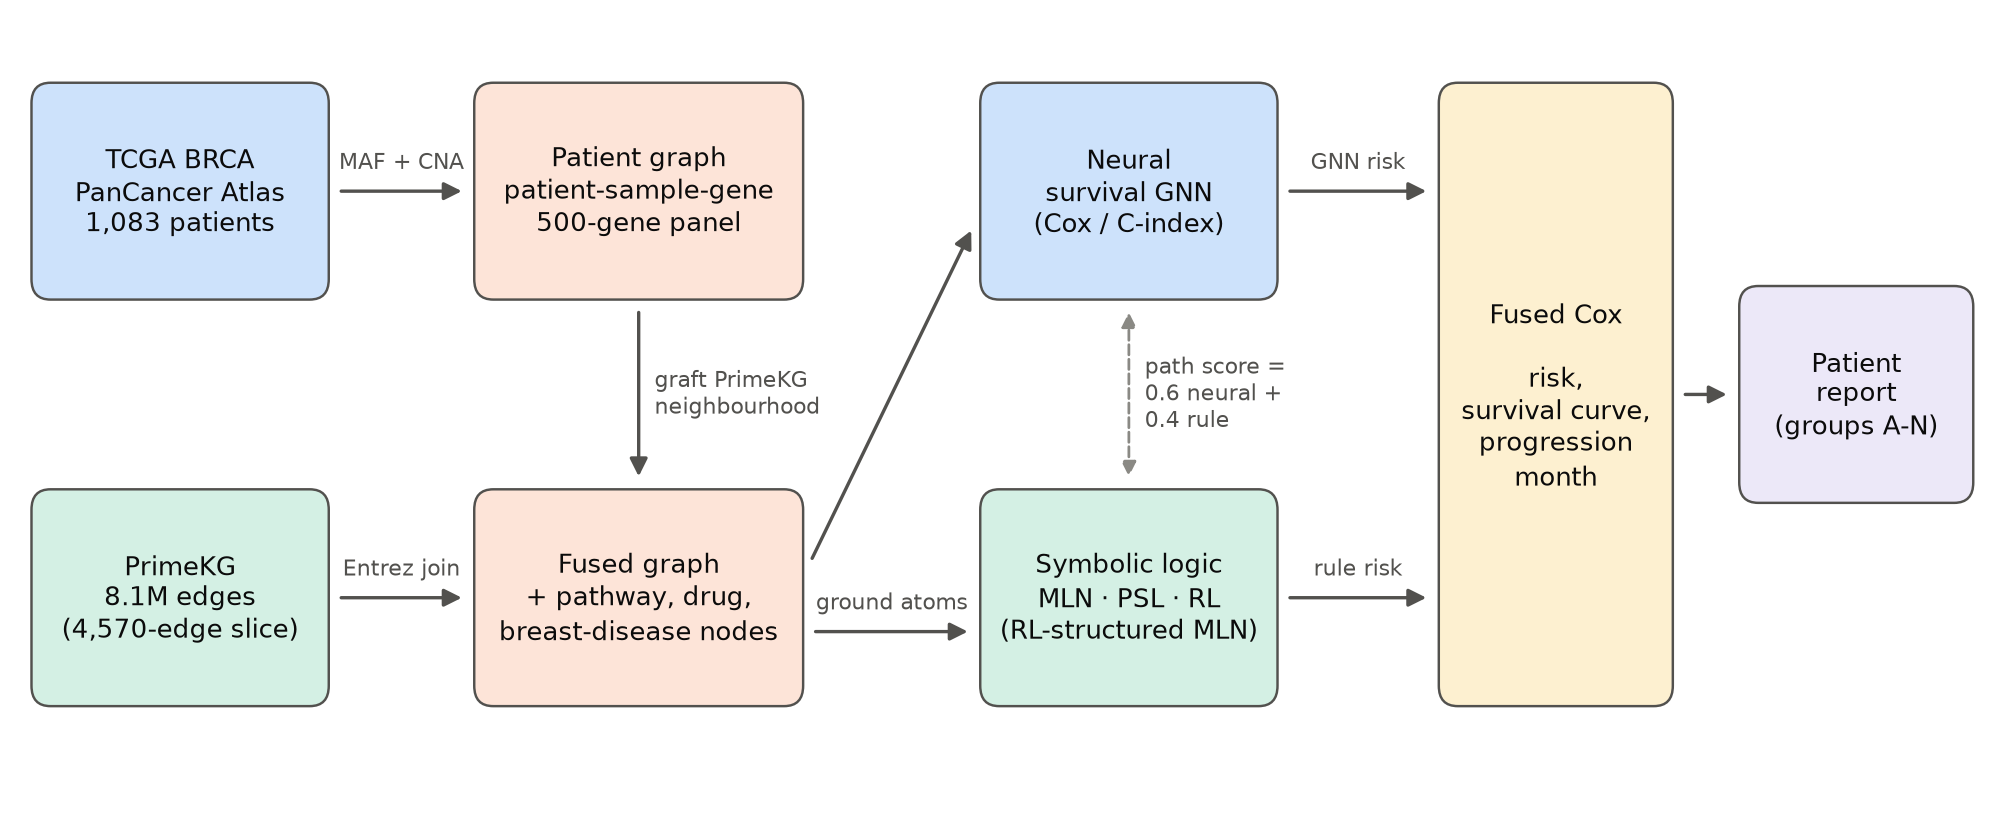
\includegraphics[width=0.93\textwidth]{fig_pipeline.png}\end{center}

\section{The flow of work, stage by stage}
\small
\begin{tabularx}{\textwidth}{>{\raggedright\bfseries}p{2.3cm}Y>{\raggedright\scriptsize\ttfamily\arraybackslash}p{4.9cm}}
\toprule
Stage & What happens & Code \\
\midrule
1. Data & Clinical, mutation, and copy-number tables from cBioPortal, checked against official checksums. Outcome columns are blocked from every input. & src/clinical.py, src/labels.py \\
2. Patient graphs & Patient $\to$ sample $\to$ altered gene, limited to a 500-gene panel with 27 known drivers. & scripts/build\_patient\_graphs.py \\
3. PrimeKG fusion & Genes join PrimeKG on Entrez ID. A 4,570-edge slice adds partners, pathways, drugs, and breast diseases (2 hops). & src/dataset\_fusion.py \\
4. Neural & Seven GNNs tested. GraphSAGE with a C-index loss gives the neural risk, and GNNExplainer scores every edge. & src/gnn\_models.py \\
5. Symbolic & 422 facts per patient. Markov logic, soft logic, and RL rules compared against RuleKit. The RL-structured survival MLN is the engine. & src/neurosymbolic/logic/ \\
6. Fusion & One Cox model on clinical fields, the GNN risk, and the logic risk. Chosen by the one-standard-error rule. & scripts/run\_neurosymbolic\_pipeline.py \\
7. Month & A log-logistic time model, fitted on past progressors, estimates the month of progression. & src/neurosymbolic/timing.py \\
8. Paths & Each path scored $0.6\times$ neural $+\ 0.4\times$ rule. The strongest 3 to 5 are shown. & src/neurosymbolic/paths.py \\
9. Reports & 1,083 PDFs in five groups by recorded progression time (A to D, and N for none). & scripts/build\_patient\_reports.py \\
\bottomrule
\end{tabularx}
\normalsize
Every prediction is out-of-fold: five-fold cross-validation with seed 42, so no patient is scored by a model that saw them.

\section{How the project evolved}
\begin{center}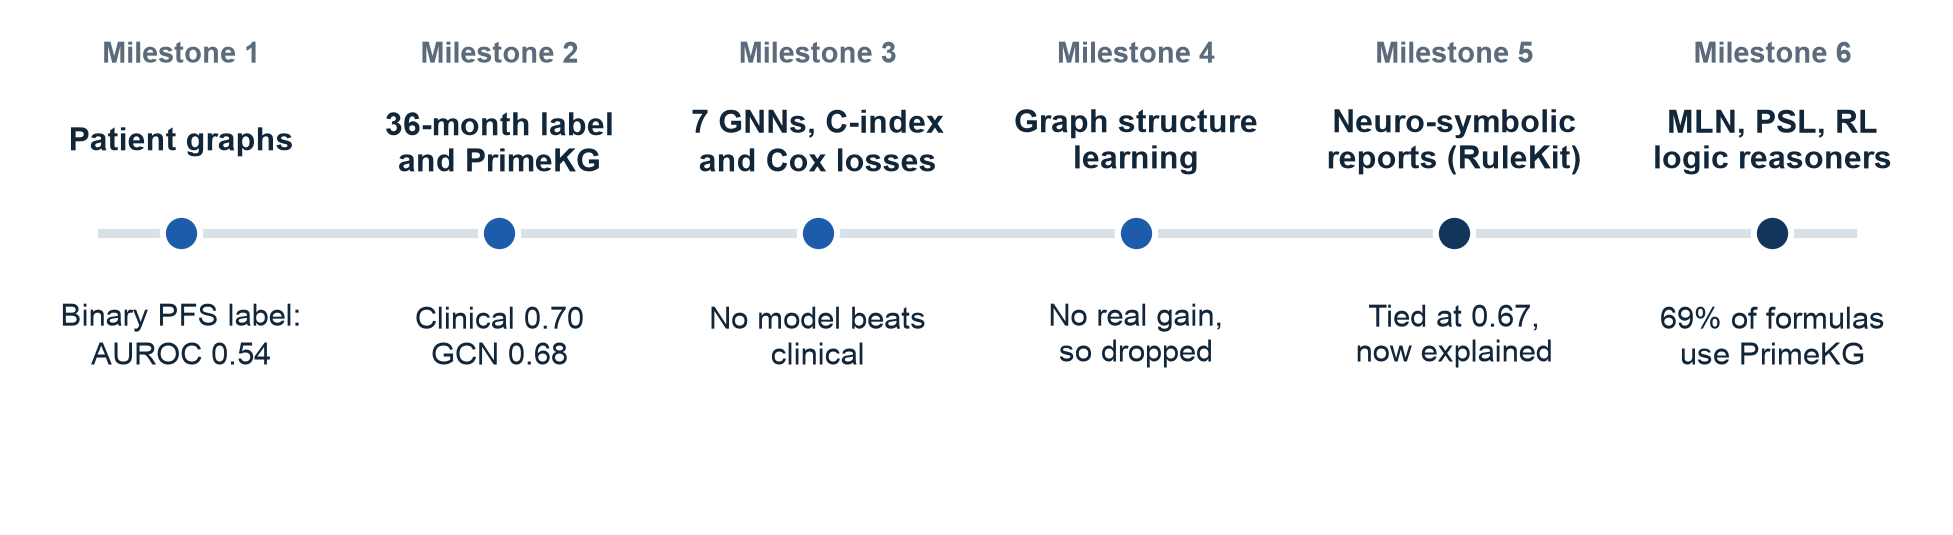
\includegraphics[width=\textwidth]{fig_timeline.png}\end{center}
\small
\begin{tabularx}{\textwidth}{>{\raggedright\bfseries}p{3.4cm}Y>{\raggedright\arraybackslash}p{3.2cm}}
\toprule
Tried & What happened & Decision \\
\midrule
Binary label on raw status & Censored patients counted as negatives, AUROC 0.54 & Replaced by 36-month label and survival losses \\
Seven GNN architectures & None beat clinical logistic regression (AUROC 0.703) & Kept GraphSAGE as the neural part \\
Graph structure learning & First version hurt GCN (AUPRC 0.396 to 0.316), second within noise & Not adopted \\
SMOTE, GSE2034 graphs, RSF & No gain, and a linear model still won & Dropped \\
RuleKit IF-THEN rules & About 8 unweighted rules per fold, 10\% using PrimeKG & Kept as baseline \\
MLN, PSL, RL, RL + MLN & Accuracy tied, but RL + MLN uses PrimeKG in 69\% of formulas & RL + MLN is the engine \\
\bottomrule
\end{tabularx}
\normalsize

\section{Results to remember}
\begin{center}
\colorbox{tint}{\parbox{0.3\textwidth}{\centering\vspace{4pt}{\Large\bfseries\color{navy}0.664}\\ \small C-index of our model, tied with clinical Cox at 0.675\vspace{4pt}}}\hfill
\colorbox{tintgreen}{\parbox{0.3\textwidth}{\centering\vspace{4pt}{\Large\bfseries\color{navy}69\%}\\ \small of logic formulas use PrimeKG, against 10\% for RuleKit\vspace{4pt}}}\hfill
\colorbox{tintred}{\parbox{0.3\textwidth}{\centering\vspace{4pt}{\Large\bfseries\color{navy}48\%}\\ \small of month estimates within 12 months, against 37\% for a guess\vspace{4pt}}}
\end{center}
Every model family stops near a C-index of 0.67. With 145 events, clinical facts carry most of the signal, so the neural and logic parts add explanation rather than accuracy.

\section{Run it}
\small
\begin{verbatim}
pip install -r requirements.txt
python scripts/run_neurosymbolic_pipeline.py         # all five stages, about 50 min
python scripts/build_patient_reports.py --workers 4  # 1,083 reports, about 5 min
python scripts/export_demo_model.py                  # export the model for the demo
python demo/build_demo.py && node demo/check_engine.js
python -m unittest discover -s tests                 # 58 tests
\end{verbatim}
\normalsize

\section{Where to find things}
\small
\begin{tabularx}{\textwidth}{>{\raggedright\scriptsize\ttfamily}p{7.0cm}Y}
\toprule
\normalfont Location & Contents \\
\midrule
outputs/patient\_reports/ & Patient reports, group summaries, and the cohort overview \\
notebooks/neurosymbolic\_patient\_reports.ipynb & Walkthrough of the whole system \\
notebooks/symbolic\_reasoning\_novelty.ipynb & The logic reasoners and the novelty \\
report/thesis.pdf & Full project report, with all equations \\
presentation/ & Panel deck, team guide, and this workflow \\
demo/index.html & Browser demo that runs the fitted model offline \\
\bottomrule
\end{tabularx}

\end{document}
